\section{Fractures and diffusion}

File: \texttt{04\_frac\_diffusion.yaml}

\subsection{Description}

In Flow123D domain interaction with fractures can be implemented. This
example comes from a study of evaluation of influence of an individual
processes (diffusion, linear sorption, dual-porosity) between domain
interaction in transport. The background of this study is movement of
contaminant mass from deep repository along fractures. The output mass
from fracture and rock is evaluated for every individual process.

The user will learn how to:

\begin{itemize}
\tightlist
\item
  prepare mesh of fractured zone
\item
  define union of mesh regions
\item
  use advection-diffusion transport model
\item
  define variable time step
\end{itemize}

\subsection{Input}

\subsubsection{Geometry and mesh generation}

The simulation area \(100 \times 100\) m is cut by two flow fractures
from which two blind fractures separate (see Figure \ref{fig:mesh}). The
cross-section of the fractures is 0.01 m.

Instead of defining a geometry with thin 2D fractures (which would yield
too large mesh), in Flow123d one can treat fractures as lines with
intrinsic cross-section area (or surfaces with intrinsic width). In
order to produce a compatible mesh, where fracture elements are faces of
triangles, we use additional GMSH command in the file
\texttt{04\_mesh.geo}:

\begin{verbatim}
  Line { 9:16 } In Surface { 20 };
\end{verbatim}

This ensures that the 2D mesh will adapt so that elements do not cross
the fracture lines (see Figure \ref{fig:mesh}).

\begin{figure}[htbp]
\centering
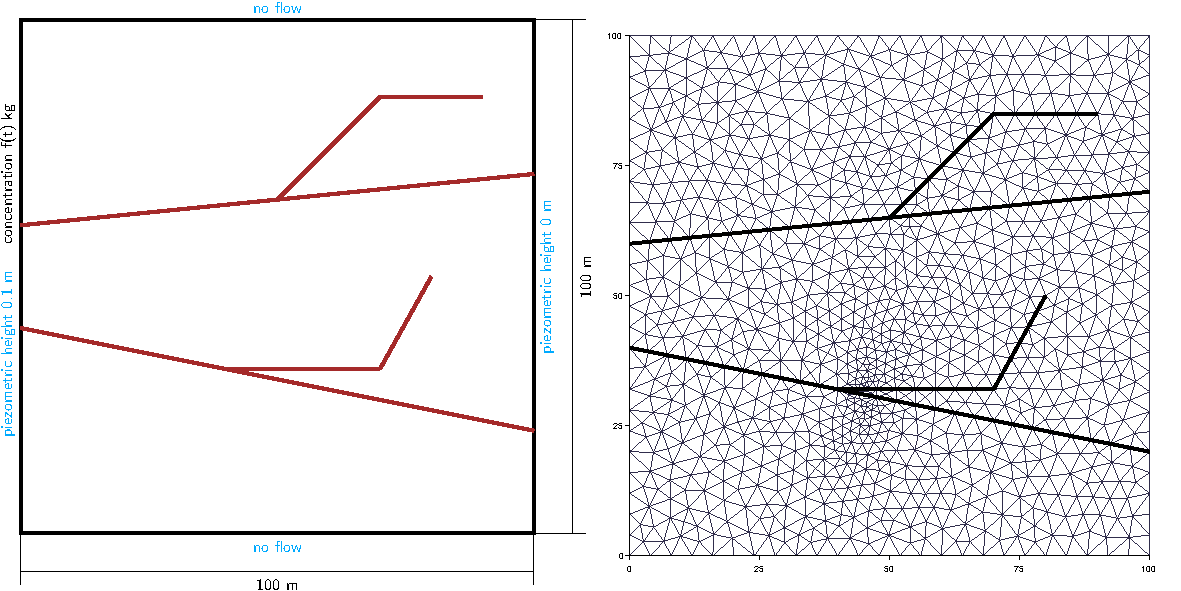
\includegraphics[width=1.00000\textwidth]{tutor_figures/04_geomesh.pdf}
\caption{Geometry and mesh of simulation area.\label{fig:mesh}}
\end{figure}

In the YAML file one can define regions in addition to those from MSH
file. We use the type \texttt{!Union} type in the array \texttt{regions}
to define sets of regions sharing some properties (e.g.~boundary
conditions):

\begin{verbatim}
mesh:
  mesh_file: 04_mesh.msh
  regions:
    - !Union
      name: flow_fractures
      regions:
        - flow_fracture1
        - flow_fracture2
    - !Union
      name: blind_fractures
      regions:
        - blind_fracture1
        - blind_fracture2
    - !Union
      name: BC_right
      regions:
        - .right
        - .right_points
    - !Union
      name: BC_left
      regions:
        - .left
        - .left_points
\end{verbatim}

\subsubsection{Hydraulic model}

We are interested in simulation for 50000 years, hence we use year as
the time units in the definition of model parameters. Hydraulic
conductivity \(k = 10^{-11}\) m/s (0.000315 m/yr) was considered for
rock massif. For the flow fractures and for the blind fractures we
considered \(k = 10^{-6}\) (31.5 m/yr) and \(k = 10^{-7}\) (3.15 m/yr),
respectively. These values are in accordance with typical values of
conductivity of a massif considered for deep repository. The thickness
of model was set to 0.01 m for fractures:

\begin{verbatim}
input_fields:
- region: rock
  conductivity: 0.000315
- region: flow_fractures
  conductivity: 31.5
  cross_section: 0.01
- region: blind_fractures
  conductivity: 3.15       # variant without blind-fractures conductivity: 0.000315
  cross_section: 0.01
\end{verbatim}

To eliminate the blind fractures from the model, one can set their
conductivity identical to the rock. Other possibility is to use the same
conductivity as in the flow-fractures.

Two dirichlet boundary conditions were defined for the flux: piezometric
head 0.1 m on the left side and 0 m on the right side:

\begin{verbatim}
- region: BC_left
  bc_type: dirichlet
  bc_piezo_head: 0.1
- region: BC_right
  bc_type: dirichlet
  bc_piezo_head: 0
\end{verbatim}

The above values were chosen in order to obtain filtration flux in the
flux-fractures approximately \(1 \times 10^{-9}\) m/s (\(\approx\) 0.1
m/yr). Other sides are nonpermeable.

\subsubsection{Transport model}

We use the advection-diffusion equation:

\begin{verbatim}
solute_equation: !Coupling_OperatorSplitting
  transport: !Solute_AdvectionDiffusion_DG
\end{verbatim}

The porosity was set to 0.005 for rock and 0.1 for fractures. The
parameters of mechanical dispersion are set to 5 m for longitudinal
dispersivity and 0.5 m for transversal dispersivity. For the molecular
diffusivity we use the same value at rock and fractures:
\(D_m = 3.69 \times 10^{-2}\) m\(^2\)/yr. Since in Flow123d the
molecular diffusion tensor has the form \(D_m\vartheta^{1/3}\mathbb I\),
the effective molecular diffusivity will be 2.7 times higher on the
fractures than in the rock (Table \ref{tbl:coefDiff}):

\begin{verbatim}
  input_fields:
  - region: rock
    init_conc: 0
    porosity: 0.005
    diff_m: 0.0369
    disp_l: 5
    disp_t: 0.5
  - region: flow_fractures
    init_conc: 0
    porosity: 0.1
    diff_m: 0.0369
    disp_l: 5
    disp_t: 0.5
  - region: blind_fractures
    init_conc: 0
    porosity: 0.1
    diff_m: 0.0369
    disp_l: 5
    disp_t: 0.5
\end{verbatim}

\begin{longtable}[c]{@{}lrr@{}}
\caption{Coefficient of molecular diffusion prescribed in Flow123d.
\label{tbl:coefDiff}}\tabularnewline
\toprule
Quantity & Rock & Fracture\tabularnewline
\midrule
\endfirsthead
\toprule
Quantity & Rock & Fracture\tabularnewline
\midrule
\endhead
Porosity \(\vartheta\) {[}\(-\){]} & 0.005 & 0.1\tabularnewline
Coefficient of molecular diffusion \(D_m\) {[}m\(^2\)/s{]} & 1e-9 &
1e-9\tabularnewline
Effective molecular diffusion \(D_m\vartheta^{1/3}\) {[}m\(^2\)/s{]} &
1.71e-10 & 4.64e-10\tabularnewline
\bottomrule
\end{longtable}

The boundary condition for the concentration at the fracture was
prescribed in the form of Gaussian curve
\[ f(t) = \frac1{20} \frac{1}{\sigma\sqrt{2\pi}}e^{-\frac12\left(\frac{t-t_0}{\sigma}\right)^2}, \]
with the meanvalue \(t_0=2000\) years and standard deviation
\(\sigma=700\) years:

\begin{verbatim}
  - region: .left_0
    bc_type: dirichlet
    bc_conc: !FieldFormula
      value: 2.84959e-5*exp(-0.5*((t-2000)/700)^2)
\end{verbatim}

It means that during the simulation time \(T=50000\) years, almost 0.05
kg/m\(^3\) (\(=\int_0^Tf(t)\,dt\)) of water is released. Maximum
concentration of realised water is 0.028 g/m\(^3\) (\(=f(t_0)\)). The
mean value corresponds with real values of release of isotopes of deep
repository.

For better resolution of the time-dependent boundary condition, we
refine the initial output time step and after 5000 years we increase it:

\begin{verbatim}
output_stream:
  times:
    - step: 500
      end: 5000
    - begin: 5000
      step: 5000
\end{verbatim}

Here \texttt{times} is an array of time grids, each having optional
parameters \texttt{begin}, \texttt{end} and \texttt{step}. The
computational time step will adapt to this grid automatically.

\subsection{Results}

The result of model with and without blind fractures (file
\texttt{04\_frac\_diffusion\_noblind.yaml}) is depicted in Figure
\ref{fig:diff_res}. We can see that with blind fractures, the water is
more contaminated at the outflow from the rock. The influence on flow
fractures is negligible.

\begin{figure}[htbp]
\centering
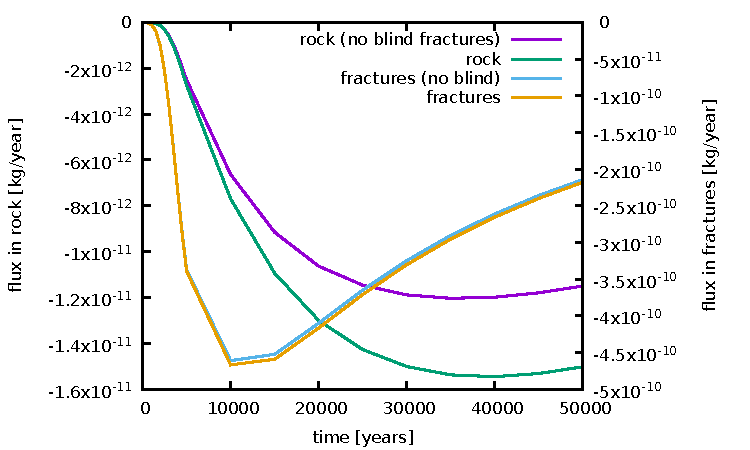
\includegraphics{tutor_figures/04_mass_flux.pdf}
\caption{Outgoing mass flux through the right part of the boundary.
Comparison of results with and without blind
fractures.\label{fig:diff_res}}
\end{figure}
